\section{Methodology}
\lhead{\leftmark}
The equipment needed and procedures undertaken to carry out 3D printing are described in the following sections. The experiment was done at iPIC (Rapid Prototyping Lab) in JKUAT.
\subsection{Equipment}
\begin{enumerate}
\item 3D Scanning hardware and software (Artec3D, Artec Spider, Artec Studio.)
\item Workpiece shown in Figure \ref{fig:3dscan}
\item 3D Printing hardware and software (Tiertime Up! Mini)
\end{enumerate}
\begin{center}
	\begin{figure}[h!]
	\centering
	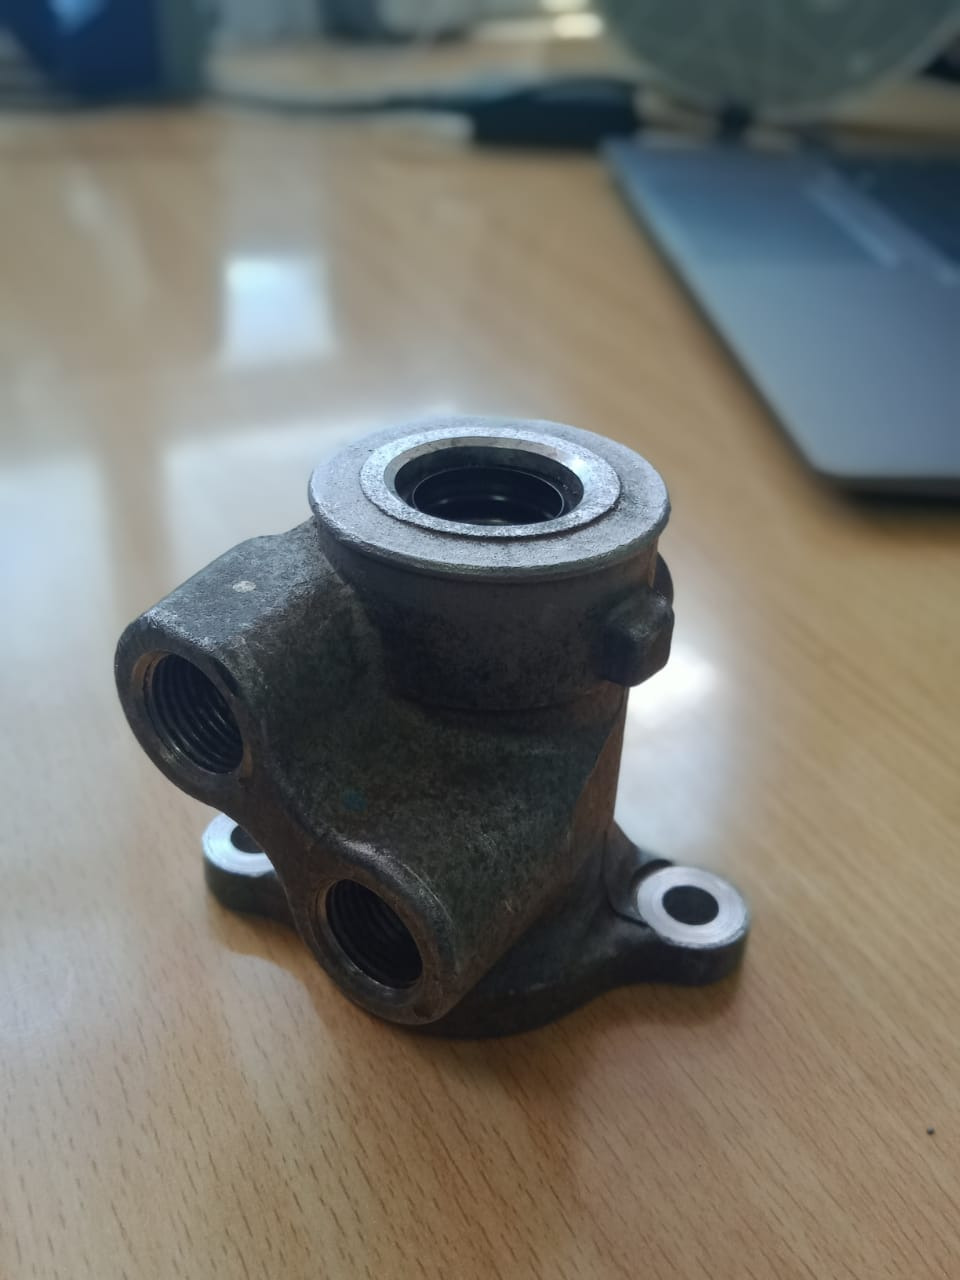
\includegraphics[width=0.4\linewidth]{Figures/Figure}
	\caption{Complex Workpiece}
	\label{fig:3dscan}
	\end{figure}
\end{center}
\newpage
\subsection{Procedure}
The 3D scanning hardware and software were set up and the workpiece placed on the turntable for scanning. Figure \ref{fig:scanning} shows the workpiece being scanned.\\
Several scans were performed and the final 3D model was obtained. Some post-processing was performed on the 3D Scan data before processing it into a 3D Model. Some of these procedures are:
\begin{enumerate}
	\item Aligning the multiple scans using various coincident points and axes on each scan.
	\item Denoising - removing noisy areas from the scan.
	\item Trimming unwanted parts from the scan.
	\item Making adjustments to distorted geometry.
\end{enumerate} 
\begin{center}
 	\begin{figure}[h!]
 	\centering
 	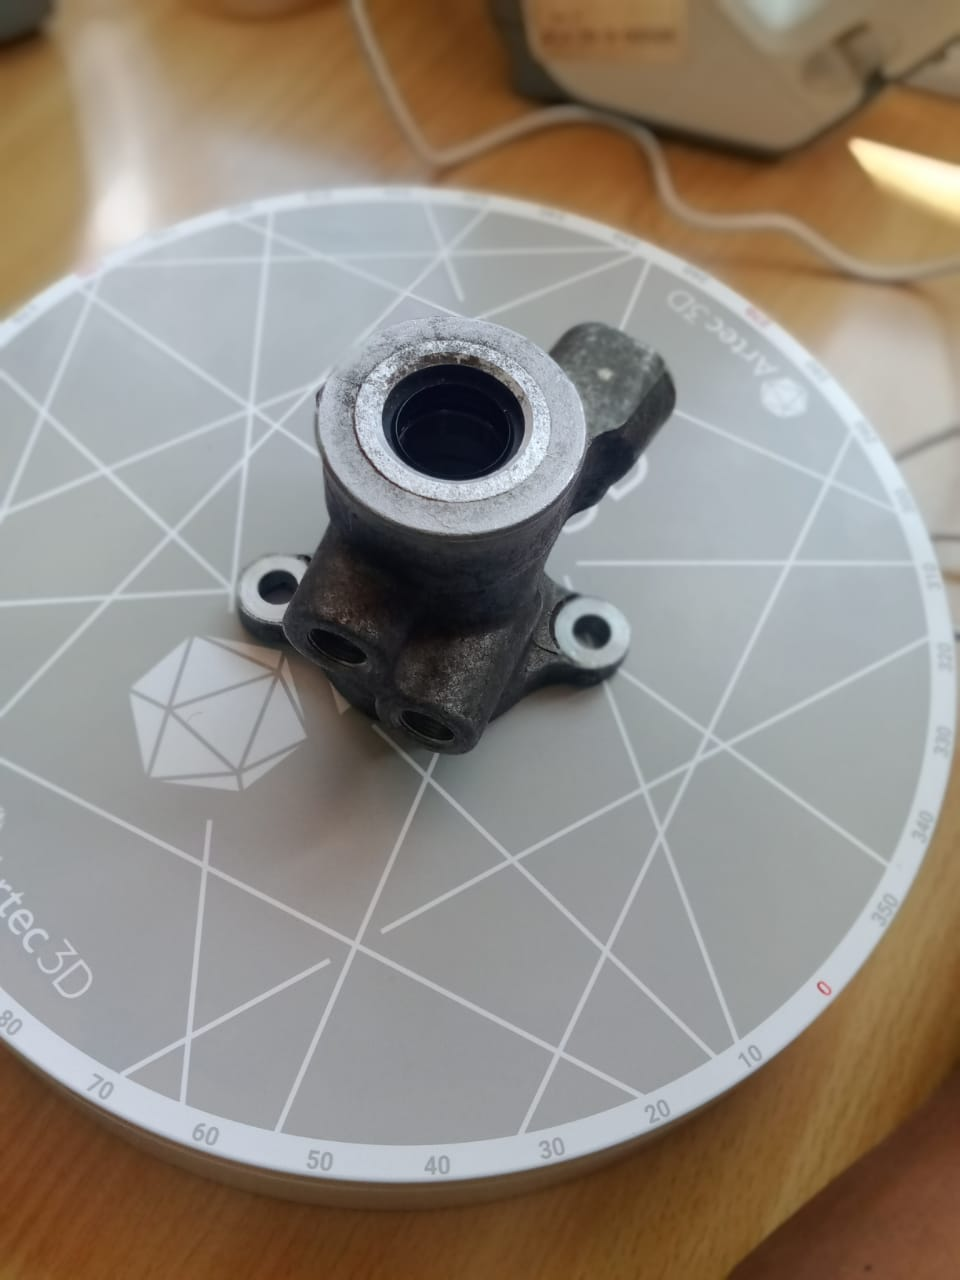
\includegraphics[width=0.4\linewidth]{Figures/Figure 2}
 	\caption[Scanning]{Workpiece being scanned}
 	\label{fig:scanning}
 	\end{figure}
 \end{center}
In this practical exercise, FDM was used to come up with a 3D object.
